\labelchapter{records}{Records, Arrays, and String}

Records, arrays, and strings are aggregate data types.  A record is
like a tuple where the elements of the tuple are named.  Arrays and
strings are fixed-length sequences of data supporting random access to
the elements in constant time.  All three types support mutation of
elements, by assignment.

\labelsection{sect-records}{Records}

\label{keyword:records}
\index{types!records}
\index{;!record field separator}
\index{\{\}@\lstinline/{ $\cdots$ }/ records}
\index{identifiers!record labels}
A record is a labeled collection of values of arbitrary types.  The
syntax for a record type is a set of field type definitions surrounded
by braces, and separated by semicolons.  Fields are declared as
\hbox{\lstinline/label : type/}, where the label is an identifier that must begin
with a lowercase letter or an underscore.  For example, the following
record redefines the database entry from Chapter~\refchapter{tuples}.

\begin{ocaml}
# type db_entry =
     { name   : string;
       height : float;
       phone  : string;
       salary : float
     };;
@
\begin{topoutput}
type db_entry = { name: string; height: float;
                  phone: string; salary: float }
\end{topoutput}
@
\end{ocaml}
%
The syntax for a record value is similar to the type declaration, but the
fields are defined as \hbox{\lstinline/label = expr/}.  Here is an example
database entry.

\begin{ocaml}
# let jason =
     { name   = "Jason";
       height = 6.25;
       phone  = "626-555-1212";
       salary = 50.0
     };;
@
\begin{topoutput}
val jason : db_entry =
  {name="Jason"; height=6.25;
   phone="626-555-1212"; salary=50}
\end{topoutput}
@
\end{ocaml}
%
\index{.!record projection}
\index{record projection}
\label{keyword:.}
There are two ways to access the fields in a record.  The
projection operation \hbox{\lstinline/r.l/} returns the field labeled \hbox{\lstinline/l/} in
record \hbox{\lstinline/r/}.

\begin{ocaml}
# jason.height;;
@
\begin{topoutput}
- : float = 6.25
\end{topoutput}
@
# jason.phone;;
@
\begin{topoutput}
- : string = "626-555-1212"
\end{topoutput}
@
\end{ocaml}
%
\label{patterns:record}
Pattern matching can also be used to access the fields of a record.
The syntax for a pattern is like a record value, but the fields
contain a label and a pattern \hbox{\lstinline/label = patt/}.  Not all of the
fields have to be included.  Note that the binding occurrences of the
variables \hbox{\lstinline/n/} and \hbox{\lstinline/h/} occur to the \emph{right} of the equality symbol
in their fields.

\begin{ocaml}
# let { name = n; height = h } = jason;;
@
\begin{topoutput}
val n : string = "Jason"
val h : float = 6.25
\end{topoutput}
@
\end{ocaml}

\labelsubsection{record-update}{Functional and imperative record updates}

\label{records:record-update}
\index{records!functional update}
\index{with@\lstinline/with/ (functional record update)}
There is a functional update operation that produces a copy of a
record with new values for the specified fields.  The syntax for
functional update uses the \hbox{\lstinline/with/} keyword in a record definition.

\begin{ocaml}
# let dave = { jason with name = "Dave"; height = 5.9 };;
@
\begin{topoutput}
val dave : db_entry =
  {name="Dave"; height=5.9; phone="626-555-1212"; salary=50}
\end{topoutput}
@
# jason;;
@
\begin{topoutput}
- : db_entry = {name="Jason"; height=6.25;
                phone="626-555-1212"; salary=50}
\end{topoutput}
@
\end{ocaml}
%
\label{keyword:mutable(records)}
\index{mutable!record fields}
Record fields can also be modified by assignment, but only if the
record field is declared as mutable in the type definition for the
record.  The syntax for a mutable field uses the \hbox{\lstinline/mutable/}
keyword before the field label.  For example, if we wanted to allow
salaries to be modified, we would need to declare the field \hbox{\lstinline/salary/}
as \hbox{\lstinline/mutable/}.

\begin{ocaml}
# type db_entry =
     { name : string;
       height : float;
       phone : string;
       mutable salary : float
     };;
@
\begin{topoutput}
type db_entry =
  { name: string;
    height: float;
    phone: string;
    mutable salary: float }
\end{topoutput}
@
# let jason =
    { name = "Jason";
      height = 6.25;
      phone = "626-555-1212";
      salary = 50.0
    };;
@
\begin{topoutput}
val jason : db_entry =
  {name="Jason"; height=6.25; phone="626-555-1212"; salary=50}
\end{topoutput}
@
\end{ocaml}
%
\label{keyword:<-(record-field-assignment)}
\index{records!field assignment}
\index{<-!record field assignment}
The syntax for a field update is \hbox{\lstinline/r.label <- expr/}.  For example,
if we want to give \hbox{\lstinline/jason/} a raise, we would use the following statement.

\begin{ocaml}
# jason.salary <- 150.0;;
@
\begin{topoutput}
- : unit = ()
\end{topoutput}
@
# jason;;
@
\begin{topoutput}
- : db_entry = {name="Jason"; height=6.25; phone="626-555-1212"; salary=150}
\end{topoutput}
@
\end{ocaml}
%
Note that the assignment statement itself returns the canonical unit
value \hbox{\lstinline/()/}.  That is, it doesn't return a useful value, unlike
the functional update.  A functional update creates a completely new
copy of a record; assignments to the copies do not interfere.

\begin{ocaml}
# let dave = { jason with name = "Dave" };;
@
\begin{topoutput}
val dave : db_entry =
  {name="Dave"; height=6.25; phone="626-555-1212"; salary=150}
\end{topoutput}
@
# dave.salary <- 180.0;;
@
\begin{topoutput}
- : unit = ()
\end{topoutput}
@
# dave;;
@
\begin{topoutput}
- : db_entry = {name="Dave"; height=6.25; phone="626-555-1212"; salary=180}
\end{topoutput}
@
# jason;;
@
\begin{topoutput}
- : db_entry = {name="Jason"; height=6.25; phone="626-555-1212"; salary=150}
\end{topoutput}
@
\end{ocaml}

\labelsubsection{record-labels}{Field label namespace}

\index{records!field namespace}
One important point: the namespace for toplevel record field labels is
flat.  This is important if you intend to declare records with the
same field names.  If you do, the original labels will be lost!  For
example, consider the following sequence.

\begin{ocaml}
# type rec1 = { name : string; height : float };;
@
\begin{topoutput}
type rec1 = { name: string; height: float }
\end{topoutput}
@
# let jason = { name = "Jason"; height = 6.25 };;
@
\begin{topoutput}
val jason : rec1 = {name="Jason"; height=6.25}
\end{topoutput}
@
# type rec2 = { name : string; phone : string };;
@
\begin{topoutput}
type rec2 = { name: string; phone: string }
\end{topoutput}
@
# let dave = { name = "Dave"; phone = "626-555-1212" };;
@
\begin{topoutput}
val dave : rec2 = {name="Dave"; phone="626-555-1212"}
\end{topoutput}
@
# jason.name;;
@
\begin{toperror}
Characters 0-5:
This expression has type rec1 but is here used with type rec2
\end{toperror}
@
# dave.name;;
@
\begin{topoutput}
- : string = "Dave"
\end{topoutput}
@
# let bob = { name = "Bob"; height = 5.75 };;
@
\begin{toperror}
Characters 10-41:
The label height belongs to the type rec1
but is here mixed with labels of type rec2
\end{toperror}
@
\end{ocaml}
%
In this case, the \hbox{\lstinline/name/} field was redefined in the
type definition for \hbox{\lstinline/rec2/}.  At this point, the
original \hbox{\lstinline/rec1.name/} label is lost, making it
impossible to access the name field in a value of type
\hbox{\lstinline/rec1/}, and impossible to construct new values of
type \hbox{\lstinline/rec1/}.  It is, however, permissible to use the
same label names in separate files, as we will see in
Chapter~\refchapter{modules}.

\labelsection{arrays}{Arrays}

\label{keyword:arrays}
\index{arrays}
\index{[ ]@\lstinline/[$\pipe \cdots \pipe$]/ arrays}
Arrays are fixed-size vectors of values.  All of the values must have
the same type.  The fields in the array can be accessed and modified
in constant time.  Arrays can be created with the syntax
%
\hbox{\lstinline/[| $e_1$; $e_2$; $\cdots$; $e_n$ |]/},
which creates an array of length $n$ initialized with
the values computed from the expressions $e_1, \ldots, e_n$.

\begin{ocaml}
# let a = [|1; 3; 5; 7|];;
@
\begin{topoutput}
val a : int array = [|1; 3; 5; 7|]
\end{topoutput}
@
\end{ocaml}
%
\label{patterns:arrays}
\label{keyword:.(}
\index{.()@\lstinline/.()/ array subscripting}
Fields can be accessed with the \hbox{\lstinline/a.(i)/} construction.  Array
indexes start from 0, and runtime checking is used to ensure that indexes are
within the array bounds.

\begin{ocaml}
# a.(0);;
@
\begin{topoutput}
- : int = 1
\end{topoutput}
@
# a.(1);;
@
\begin{topoutput}
- : int = 3
\end{topoutput}
@
# a.(5);;
@
\begin{topoutput}
Uncaught exception: Invalid_argument("Array.get")
\end{topoutput}
@
\end{ocaml}
%
\label{keyword:<-(array-field-assignment)}
\index{<-!array field assignment}
Fields are updated with the \hbox{\lstinline/a.(i) <- e/} assignment
statement.

\begin{ocaml}
# a.(2) <- 9;;
@
\begin{topoutput}
- : unit = ()
\end{topoutput}
@
# a;;
@
\begin{topoutput}
- : int array = [|1; 3; 9; 7|]
\end{topoutput}
@
\end{ocaml}
%
\index{Array module!length@\lstinline/length/}
The \hbox{\lstinline/Array/} library module defines additional functions on arrays.
Arrays of arbitrary length can be created with the \hbox{\lstinline/Array.create/}
function, which requires a length and initializer argument.  The
\hbox{\lstinline/Array.length/} function returns the number of elements in the
array.

\begin{ocaml}
# let a = Array.create 10 1;;
@
\begin{topoutput}
val a : int array = [|1; 1; 1; 1; 1; 1; 1; 1; 1; 1|]
\end{topoutput}
@
# Array.length a;;
@
\begin{topoutput}
- : int = 10
\end{topoutput}
@
\end{ocaml}
%
\index{Array module!blit@\lstinline/blit/}
The \hbox{\lstinline/Array.blit/} function can be used to copy elements
destructively from one array to another.  The \hbox{\lstinline/blit/} function
requires five arguments: the source array, a starting offset into the
array, the destination array, a starting offset into the destination
array, and the number of elements to copy.

\begin{ocaml}
# Array.blit [| 3; 4; 5; 6 |] 1 a 3 2;;
@
\begin{topoutput}
- : unit = ()
\end{topoutput}
@
# a;;
@
\begin{topoutput}
- : int array = [|1; 1; 1; 4; 5; 1; 1; 1; 1; 1|]
\end{topoutput}
@
\end{ocaml}

\labelsection{strings}{Strings}

\label{keyword:string-subscript}
\label{keyword:<-(string-assignment)}
\index{strings}
\index{.[@\lstinline/.[]/ string subscripting}
\index{<-!string assignment}
In OCaml, strings are a lot like packed arrays of characters.  The
access and update operations use the syntax \hbox{\lstinline/s.[i]/} and
\hbox{\lstinline/s.[i] <- c/}.

\begin{ocaml}
# let s = "Jason";;
@
\begin{topoutput}
val s : string = "Jason"
\end{topoutput}
@
# s.[2];;
@
\begin{topoutput}
- : char = 's'
\end{topoutput}
@
# s.[3] <- 'y';;
@
\begin{topoutput}
- : unit = ()
\end{topoutput}
@
# s;;
@
\begin{topoutput}
- : string = "Jasyn"
\end{topoutput}
@
\end{ocaml}
%
\index{String module!length@\lstinline/length/}
\index{String module!blit@\lstinline/blit/}
The \hbox{\lstinline/String/} module defines additional functions, including the
\hbox{\lstinline/String.length/} and \hbox{\lstinline/String.blit/} functions that parallel
the corresponding \hbox{\lstinline/Array/} operations.  The \hbox{\lstinline/String.create/}
function does not require an initializer.  It creates a string with
arbitrary contents.

\begin{ocaml}
# String.create 10;;
@
\begin{topoutput}
- : string = "\000\011\000\000,\200\027x\000\000"
\end{topoutput}
@
# String.create 10;;
@
\begin{topoutput}
- : string = "\196\181\027x\001\000\000\000\000\000"
\end{topoutput}
@
\end{ocaml}

\labelsection{hash-tables}{Hash tables}

To illustrate these types in action, let's implement (yet another)
dictionary, this time in the form of a hash table.  A \emph{hash
table} provides the usual map from keys to values, but this time the
expected running time for lookup and insertion is constant.  The hash table
works by computing an integer \emph{hash} of a key that serves as an
index into an array of dictionary entries.  Insertion is performed by
adding a new entry to the table at the hash index of the key; lookup
is performed by searching for an entry with a matching key at the
key's hash index.  An example of a hash table is shown in
Figure~\ref{figure:hash-table}.

\begin{figure}
\centerline{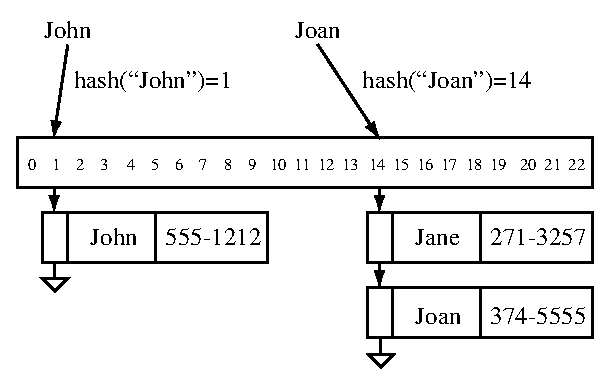
\includegraphics{hash}}
\caption{An open hash table.}
\label{figure:hash-table}
\end{figure}

In the usual case, the space of indices is smaller than the space of
keys, so hash \emph{collisions} may occur where two keys hash to the
same index.  Hash collisions can have a significant impact on
performance.  The hash table in the figure shows a so-called
``chained'' implementation, where entries with the same hash are
stored in a list associated with that index.

For our example, we'll implement a simple hash table where the keys
are strings, and the table is polymorphic over the type of values.
One approach to producing a fast, fairly good hash is called
a \emph{s-box} (for \emph{substitution box}), which uses a table of
randomly-generated numbers.

\begin{ocamlblock}
\begin{ocamlblocksize}
\begin{lstlisting}[name=hash]
let random_numbers =
   [|0x04a018c6; 0x5ba7b0f2; 0x04dcf08b; 0x1e5a22cc; 0x2523b9ea; $\cdots$|]
let random_length = Array.length random_numbers

type hash_info = { mutable hash_index : int; mutable hash_value : int }

let hash_char info c =
   let i = Char.code c in
   let index = (info.hash_index + i + 1) mod random_length in
   info.hash_value <- (info.hash_value * 3) lxor random_numbers.(index);
   info.hash_index <- index
\end{lstlisting}
\end{ocamlblocksize}
%
The record type \hbox{\lstinline/hash_info/} has two fields:
the \hbox{\lstinline/hash_index/} is an index into the random number array,
and \hbox{\lstinline/hash_value/} is the partially computed hash.  The
function \hbox{\lstinline/hash_char/} uses the character to update
the \hbox{\lstinline/hash_index/} and updates the \hbox{\lstinline/hash_value/} by
taking the exclusive-or with a random integer.  The hash of a string
is computed one character at a time.

\begin{ocamlblocksize}
\begin{lstlisting}[name=hash]
let hash s =
   let info = { hash_index = 0; hash_value = 0 } in
   for i = 0 to String.length s - 1 do
      hash_char info s.[i]
   done;
   info.hash_value
\end{lstlisting}
\end{ocamlblocksize}
%
Note that the bounds in the for-loop on line 3 are \emph{inclusive};
the index of the first character in the string is \hbox{\lstinline/0/}, and
the final character has index \hbox{\lstinline/String.length s - 1/}.

The hash table itself is an array of key/value pair lists
(called \emph{buckets}), as shown in the following code.

\begin{ocamlblocksize}
\begin{lstlisting}[name=hash]
type 'a hash_entry = { key : string; value : 'a }
type 'a hash_table = 'a hash_entry list array

(* create : unit -> 'a hash_table *)
let create () =
   Array.create 101 []

(* add : 'a hash_table -> string -> 'a -> unit *)
let add table key value =
   let index = (hash key) mod (Array.length table) in
   table.(index) <- { key = key; value = value } :: table.(index)

(* find : 'a hash_table -> string -> 'a *)
let rec find_entry key = function
   { key = key'; value = value } :: _ when key' = key -> value
 | _ :: entries -> find_entry key entries
 | [] -> raise Not_found

let find table key =
   let index = (hash key) mod (Array.length table) in
   find_entry key table.(index)
\end{lstlisting}
\end{ocamlblocksize}
\end{ocamlblock}
%
The function
\hbox{\lstinline/add : 'a hash_table -> string -> 'a -> unit/} adds a new
entry to the table by adding the key/value pair to the table at the
hash index for the key.  The function
\hbox{\lstinline/find : 'a hash_table -> string -> 'a/}
searches the table for the entry containing the key.
